\documentclass[]{article}
\usepackage{lmodern}
\usepackage{amssymb,amsmath}
\usepackage{ifxetex,ifluatex}
\usepackage{fixltx2e} % provides \textsubscript
\ifnum 0\ifxetex 1\fi\ifluatex 1\fi=0 % if pdftex
  \usepackage[T1]{fontenc}
  \usepackage[utf8]{inputenc}
\else % if luatex or xelatex
  \ifxetex
    \usepackage{mathspec}
  \else
    \usepackage{fontspec}
  \fi
  \defaultfontfeatures{Ligatures=TeX,Scale=MatchLowercase}
\fi
% use upquote if available, for straight quotes in verbatim environments
\IfFileExists{upquote.sty}{\usepackage{upquote}}{}
% use microtype if available
\IfFileExists{microtype.sty}{%
\usepackage{microtype}
\UseMicrotypeSet[protrusion]{basicmath} % disable protrusion for tt fonts
}{}
\usepackage[margin=1in]{geometry}
\usepackage{hyperref}
\hypersetup{unicode=true,
            pdftitle={Lionfish Cluster Plot},
            pdfauthor={GG},
            pdfborder={0 0 0},
            breaklinks=true}
\urlstyle{same}  % don't use monospace font for urls
\usepackage{color}
\usepackage{fancyvrb}
\newcommand{\VerbBar}{|}
\newcommand{\VERB}{\Verb[commandchars=\\\{\}]}
\DefineVerbatimEnvironment{Highlighting}{Verbatim}{commandchars=\\\{\}}
% Add ',fontsize=\small' for more characters per line
\usepackage{framed}
\definecolor{shadecolor}{RGB}{248,248,248}
\newenvironment{Shaded}{\begin{snugshade}}{\end{snugshade}}
\newcommand{\KeywordTok}[1]{\textcolor[rgb]{0.13,0.29,0.53}{\textbf{#1}}}
\newcommand{\DataTypeTok}[1]{\textcolor[rgb]{0.13,0.29,0.53}{#1}}
\newcommand{\DecValTok}[1]{\textcolor[rgb]{0.00,0.00,0.81}{#1}}
\newcommand{\BaseNTok}[1]{\textcolor[rgb]{0.00,0.00,0.81}{#1}}
\newcommand{\FloatTok}[1]{\textcolor[rgb]{0.00,0.00,0.81}{#1}}
\newcommand{\ConstantTok}[1]{\textcolor[rgb]{0.00,0.00,0.00}{#1}}
\newcommand{\CharTok}[1]{\textcolor[rgb]{0.31,0.60,0.02}{#1}}
\newcommand{\SpecialCharTok}[1]{\textcolor[rgb]{0.00,0.00,0.00}{#1}}
\newcommand{\StringTok}[1]{\textcolor[rgb]{0.31,0.60,0.02}{#1}}
\newcommand{\VerbatimStringTok}[1]{\textcolor[rgb]{0.31,0.60,0.02}{#1}}
\newcommand{\SpecialStringTok}[1]{\textcolor[rgb]{0.31,0.60,0.02}{#1}}
\newcommand{\ImportTok}[1]{#1}
\newcommand{\CommentTok}[1]{\textcolor[rgb]{0.56,0.35,0.01}{\textit{#1}}}
\newcommand{\DocumentationTok}[1]{\textcolor[rgb]{0.56,0.35,0.01}{\textbf{\textit{#1}}}}
\newcommand{\AnnotationTok}[1]{\textcolor[rgb]{0.56,0.35,0.01}{\textbf{\textit{#1}}}}
\newcommand{\CommentVarTok}[1]{\textcolor[rgb]{0.56,0.35,0.01}{\textbf{\textit{#1}}}}
\newcommand{\OtherTok}[1]{\textcolor[rgb]{0.56,0.35,0.01}{#1}}
\newcommand{\FunctionTok}[1]{\textcolor[rgb]{0.00,0.00,0.00}{#1}}
\newcommand{\VariableTok}[1]{\textcolor[rgb]{0.00,0.00,0.00}{#1}}
\newcommand{\ControlFlowTok}[1]{\textcolor[rgb]{0.13,0.29,0.53}{\textbf{#1}}}
\newcommand{\OperatorTok}[1]{\textcolor[rgb]{0.81,0.36,0.00}{\textbf{#1}}}
\newcommand{\BuiltInTok}[1]{#1}
\newcommand{\ExtensionTok}[1]{#1}
\newcommand{\PreprocessorTok}[1]{\textcolor[rgb]{0.56,0.35,0.01}{\textit{#1}}}
\newcommand{\AttributeTok}[1]{\textcolor[rgb]{0.77,0.63,0.00}{#1}}
\newcommand{\RegionMarkerTok}[1]{#1}
\newcommand{\InformationTok}[1]{\textcolor[rgb]{0.56,0.35,0.01}{\textbf{\textit{#1}}}}
\newcommand{\WarningTok}[1]{\textcolor[rgb]{0.56,0.35,0.01}{\textbf{\textit{#1}}}}
\newcommand{\AlertTok}[1]{\textcolor[rgb]{0.94,0.16,0.16}{#1}}
\newcommand{\ErrorTok}[1]{\textcolor[rgb]{0.64,0.00,0.00}{\textbf{#1}}}
\newcommand{\NormalTok}[1]{#1}
\usepackage{graphicx,grffile}
\makeatletter
\def\maxwidth{\ifdim\Gin@nat@width>\linewidth\linewidth\else\Gin@nat@width\fi}
\def\maxheight{\ifdim\Gin@nat@height>\textheight\textheight\else\Gin@nat@height\fi}
\makeatother
% Scale images if necessary, so that they will not overflow the page
% margins by default, and it is still possible to overwrite the defaults
% using explicit options in \includegraphics[width, height, ...]{}
\setkeys{Gin}{width=\maxwidth,height=\maxheight,keepaspectratio}
\IfFileExists{parskip.sty}{%
\usepackage{parskip}
}{% else
\setlength{\parindent}{0pt}
\setlength{\parskip}{6pt plus 2pt minus 1pt}
}
\setlength{\emergencystretch}{3em}  % prevent overfull lines
\providecommand{\tightlist}{%
  \setlength{\itemsep}{0pt}\setlength{\parskip}{0pt}}
\setcounter{secnumdepth}{0}
% Redefines (sub)paragraphs to behave more like sections
\ifx\paragraph\undefined\else
\let\oldparagraph\paragraph
\renewcommand{\paragraph}[1]{\oldparagraph{#1}\mbox{}}
\fi
\ifx\subparagraph\undefined\else
\let\oldsubparagraph\subparagraph
\renewcommand{\subparagraph}[1]{\oldsubparagraph{#1}\mbox{}}
\fi

%%% Use protect on footnotes to avoid problems with footnotes in titles
\let\rmarkdownfootnote\footnote%
\def\footnote{\protect\rmarkdownfootnote}

%%% Change title format to be more compact
\usepackage{titling}

% Create subtitle command for use in maketitle
\newcommand{\subtitle}[1]{
  \posttitle{
    \begin{center}\large#1\end{center}
    }
}

\setlength{\droptitle}{-2em}
  \title{Lionfish Cluster Plot}
  \pretitle{\vspace{\droptitle}\centering\huge}
  \posttitle{\par}
  \author{GG}
  \preauthor{\centering\large\emph}
  \postauthor{\par}
  \predate{\centering\large\emph}
  \postdate{\par}
  \date{1/28/2019}


\begin{document}
\maketitle

\begin{Shaded}
\begin{Highlighting}[]
\KeywordTok{library}\NormalTok{(vegan)}
\end{Highlighting}
\end{Shaded}

\begin{verbatim}
## Warning: package 'vegan' was built under R version 3.4.4
\end{verbatim}

\begin{verbatim}
## Loading required package: permute
\end{verbatim}

\begin{verbatim}
## Loading required package: lattice
\end{verbatim}

\begin{verbatim}
## This is vegan 2.5-1
\end{verbatim}

\begin{Shaded}
\begin{Highlighting}[]
\KeywordTok{library}\NormalTok{(dbplyr)}
\KeywordTok{library}\NormalTok{(tidyverse)}
\end{Highlighting}
\end{Shaded}

\begin{verbatim}
## -- Attaching packages ------------------------------------------------------------------------------------------ tidyverse 1.2.1 --
\end{verbatim}

\begin{verbatim}
## √ ggplot2 2.2.1     √ purrr   0.2.4
## √ tibble  1.4.2     √ dplyr   0.7.4
## √ tidyr   0.8.0     √ stringr 1.3.0
## √ readr   1.1.1     √ forcats 0.3.0
\end{verbatim}

\begin{verbatim}
## -- Conflicts --------------------------------------------------------------------------------------------- tidyverse_conflicts() --
## x dplyr::filter() masks stats::filter()
## x dplyr::ident()  masks dbplyr::ident()
## x dplyr::lag()    masks stats::lag()
## x dplyr::sql()    masks dbplyr::sql()
\end{verbatim}

\begin{Shaded}
\begin{Highlighting}[]
\NormalTok{PCA_fish <-}\StringTok{ }\KeywordTok{read_csv}\NormalTok{(}\StringTok{"~/Desktop/Lionfish/Darwin_matrix.csv"}\NormalTok{)}
\end{Highlighting}
\end{Shaded}

\begin{verbatim}
## Warning: Missing column names filled in: 'X1' [1]
\end{verbatim}

\begin{verbatim}
## Parsed with column specification:
## cols(
##   .default = col_double(),
##   X1 = col_character()
## )
\end{verbatim}

\begin{verbatim}
## See spec(...) for full column specifications.
\end{verbatim}

\begin{Shaded}
\begin{Highlighting}[]
\KeywordTok{library}\NormalTok{(tidyverse)}
\KeywordTok{row.names}\NormalTok{(PCA_fish) <-}\StringTok{ }\NormalTok{PCA_fish}\OperatorTok{$}\NormalTok{X1}
\end{Highlighting}
\end{Shaded}

\begin{verbatim}
## Warning: Setting row names on a tibble is deprecated.
\end{verbatim}

\begin{Shaded}
\begin{Highlighting}[]
\NormalTok{PCA_fish[}\DecValTok{1}\NormalTok{] =}\StringTok{ }\OtherTok{NULL}
\end{Highlighting}
\end{Shaded}

K means cluster analysis

\begin{Shaded}
\begin{Highlighting}[]
\KeywordTok{library}\NormalTok{(tidyverse)  }\CommentTok{# data manipulation}
\KeywordTok{library}\NormalTok{(cluster)    }\CommentTok{# clustering algorithms}
\KeywordTok{library}\NormalTok{(factoextra)}
\end{Highlighting}
\end{Shaded}

\begin{verbatim}
## Welcome! Related Books: `Practical Guide To Cluster Analysis in R` at https://goo.gl/13EFCZ
\end{verbatim}

\begin{Shaded}
\begin{Highlighting}[]
\KeywordTok{library}\NormalTok{(ggplot2)}
\NormalTok{cluster2 <-}\StringTok{ }\KeywordTok{kmeans}\NormalTok{(PCA_fish, }\DataTypeTok{centers =} \DecValTok{2}\NormalTok{, }\DataTypeTok{nstart =} \DecValTok{25}\NormalTok{)}
\KeywordTok{str}\NormalTok{(cluster2)}
\end{Highlighting}
\end{Shaded}

\begin{verbatim}
## List of 9
##  $ cluster     : Named int [1:11] 1 1 1 1 1 2 2 2 1 2 ...
##   ..- attr(*, "names")= chr [1:11] "Elbow" "Tiger" "XL" "Spittal" ...
##  $ centers     : num [1:2, 1:29] 0.0773 0.4283 0.3028 0.0669 0.1872 ...
##   ..- attr(*, "dimnames")=List of 2
##   .. ..$ : chr [1:2] "1" "2"
##   .. ..$ : chr [1:29] "Chromis bermudae" "Chromis insolata" "Paranthia furcifer" "Chaetodon sedentarius" ...
##  $ totss       : num 1.56
##  $ withinss    : num [1:2] 0.851 0.171
##  $ tot.withinss: num 1.02
##  $ betweenss   : num 0.539
##  $ size        : int [1:2] 7 4
##  $ iter        : int 1
##  $ ifault      : int 0
##  - attr(*, "class")= chr "kmeans"
\end{verbatim}

\begin{Shaded}
\begin{Highlighting}[]
\NormalTok{pcaplot <-}\StringTok{ }\KeywordTok{fviz_cluster}\NormalTok{(cluster2, }\DataTypeTok{data =}\NormalTok{ PCA_fish, }\DataTypeTok{fill =} \StringTok{"darkblue"}\NormalTok{) }\OperatorTok{+}\StringTok{ }\KeywordTok{ylim}\NormalTok{(}\OperatorTok{-}\FloatTok{2.5}\NormalTok{,}\FloatTok{4.5}\NormalTok{) }\OperatorTok{+}\StringTok{ }\KeywordTok{theme_classic}\NormalTok{()}
\KeywordTok{ggsave}\NormalTok{(PCA_fish, }\DataTypeTok{plot =}\NormalTok{ pcaplot, }\DataTypeTok{device =} \StringTok{"eps"}\NormalTok{)}
\end{Highlighting}
\end{Shaded}

\begin{verbatim}
## Saving 6.5 x 4.5 in image
\end{verbatim}

\begin{verbatim}
## Warning in grid.Call.graphics(C_polygon, x$x, x$y, index): semi-
## transparency is not supported on this device: reported only once per page
\end{verbatim}

\begin{Shaded}
\begin{Highlighting}[]
\NormalTok{pcaplot}
\end{Highlighting}
\end{Shaded}

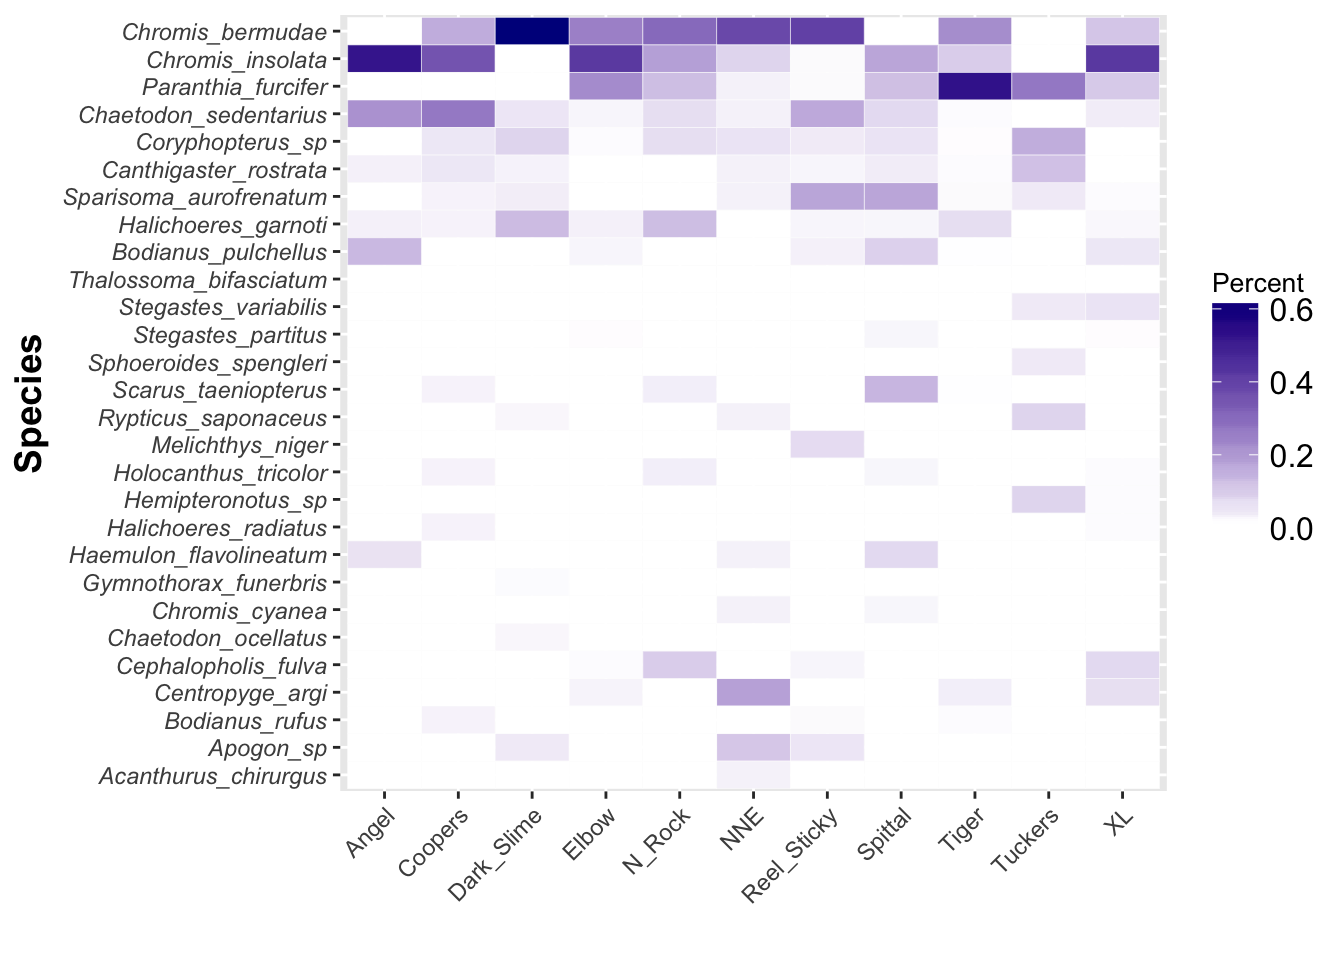
\includegraphics{Lionfish_final_cluster_analysis_files/figure-latex/unnamed-chunk-5-1.pdf}

\begin{Shaded}
\begin{Highlighting}[]
\NormalTok{ggpcaplot <-}\StringTok{ }\NormalTok{pcaplot }\OperatorTok{+}\StringTok{ }\KeywordTok{theme_classic}\NormalTok{() }\OperatorTok{+}\StringTok{ }\KeywordTok{labs}\NormalTok{(}\DataTypeTok{title=}\StringTok{""}\NormalTok{)}
\NormalTok{ggpcaplot}
\end{Highlighting}
\end{Shaded}

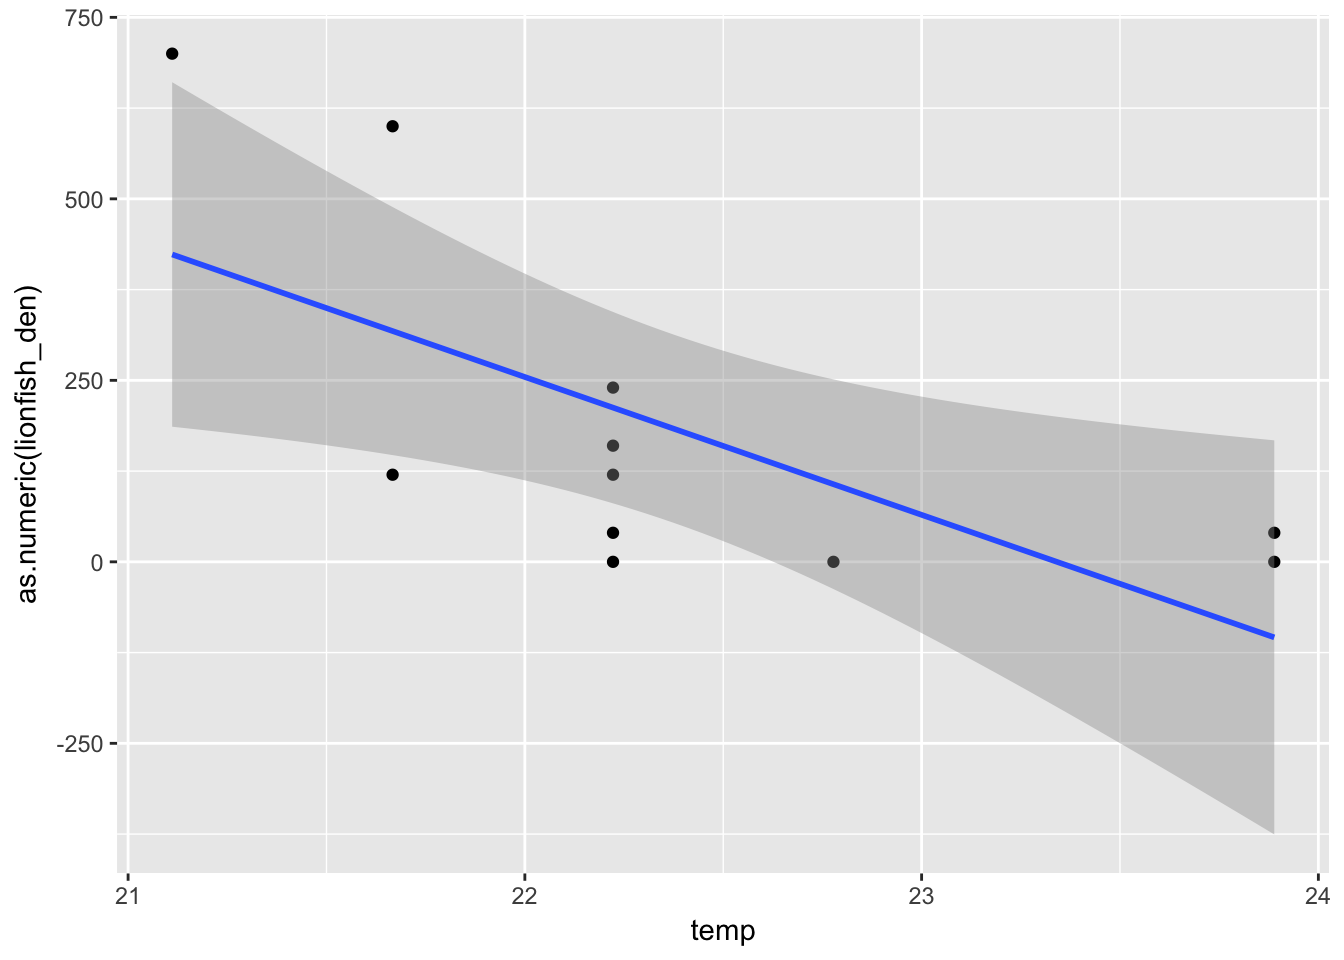
\includegraphics{Lionfish_final_cluster_analysis_files/figure-latex/unnamed-chunk-6-1.pdf}

\begin{Shaded}
\begin{Highlighting}[]
\KeywordTok{ggsave}\NormalTok{(PCA_fish, }\DataTypeTok{plot =}\NormalTok{ ggpcaplot, }\DataTypeTok{device =} \StringTok{"eps"}\NormalTok{)}
\end{Highlighting}
\end{Shaded}

\begin{verbatim}
## Saving 6.5 x 4.5 in image
\end{verbatim}

\begin{verbatim}
## Warning in grid.Call.graphics(C_polygon, x$x, x$y, index): semi-
## transparency is not supported on this device: reported only once per page
\end{verbatim}

\begin{Shaded}
\begin{Highlighting}[]
\NormalTok{cluster3 <-}\StringTok{ }\KeywordTok{kmeans}\NormalTok{(PCA_fish, }\DataTypeTok{centers =} \DecValTok{3}\NormalTok{, }\DataTypeTok{nstart =} \DecValTok{25}\NormalTok{)}
\KeywordTok{str}\NormalTok{(cluster3)}
\end{Highlighting}
\end{Shaded}

\begin{verbatim}
## List of 9
##  $ cluster     : Named int [1:11] 1 3 1 1 1 2 2 2 1 2 ...
##   ..- attr(*, "names")= chr [1:11] "Elbow" "Tiger" "XL" "Spittal" ...
##  $ centers     : num [1:3, 1:29] 0.0895 0.4283 0.0469 0.3991 0.0669 ...
##   ..- attr(*, "dimnames")=List of 2
##   .. ..$ : chr [1:3] "1" "2" "3"
##   .. ..$ : chr [1:29] "Chromis bermudae" "Chromis insolata" "Paranthia furcifer" "Chaetodon sedentarius" ...
##  $ totss       : num 1.56
##  $ withinss    : num [1:3] 0.298 0.171 0.129
##  $ tot.withinss: num 0.598
##  $ betweenss   : num 0.964
##  $ size        : int [1:3] 5 4 2
##  $ iter        : int 1
##  $ ifault      : int 0
##  - attr(*, "class")= chr "kmeans"
\end{verbatim}

\begin{Shaded}
\begin{Highlighting}[]
\KeywordTok{fviz_cluster}\NormalTok{(cluster3, }\DataTypeTok{data =}\NormalTok{ PCA_fish, }\DataTypeTok{fill =} \StringTok{"darkblue"}\NormalTok{) }\OperatorTok{+}\StringTok{ }\KeywordTok{ylim}\NormalTok{(}\OperatorTok{-}\FloatTok{2.5}\NormalTok{,}\FloatTok{4.5}\NormalTok{) }\OperatorTok{+}\StringTok{ }\KeywordTok{theme_classic}\NormalTok{()}
\end{Highlighting}
\end{Shaded}

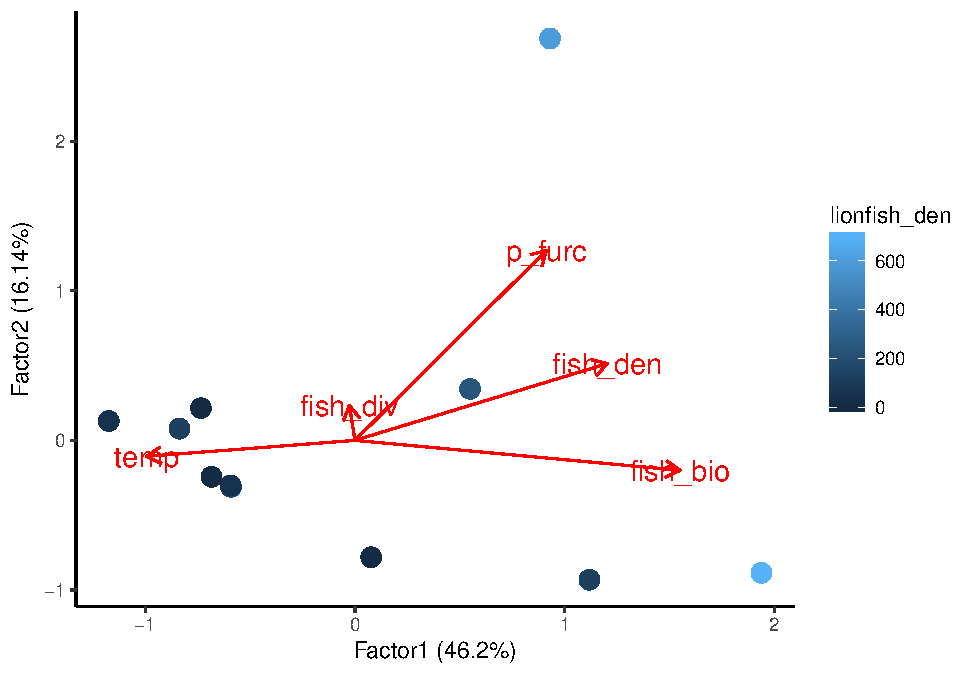
\includegraphics{Lionfish_final_cluster_analysis_files/figure-latex/unnamed-chunk-7-1.pdf}

\begin{Shaded}
\begin{Highlighting}[]
\KeywordTok{citation}\NormalTok{(}\DataTypeTok{package =} \StringTok{"vegan"}\NormalTok{)}
\end{Highlighting}
\end{Shaded}

\begin{verbatim}
## 
## To cite package 'vegan' in publications use:
## 
##   Jari Oksanen, F. Guillaume Blanchet, Michael Friendly, Roeland
##   Kindt, Pierre Legendre, Dan McGlinn, Peter R. Minchin, R. B.
##   O'Hara, Gavin L. Simpson, Peter Solymos, M. Henry H. Stevens,
##   Eduard Szoecs and Helene Wagner (2018). vegan: Community Ecology
##   Package. R package version 2.5-1.
##   https://CRAN.R-project.org/package=vegan
## 
## A BibTeX entry for LaTeX users is
## 
##   @Manual{,
##     title = {vegan: Community Ecology Package},
##     author = {Jari Oksanen and F. Guillaume Blanchet and Michael Friendly and Roeland Kindt and Pierre Legendre and Dan McGlinn and Peter R. Minchin and R. B. O'Hara and Gavin L. Simpson and Peter Solymos and M. Henry H. Stevens and Eduard Szoecs and Helene Wagner},
##     year = {2018},
##     note = {R package version 2.5-1},
##     url = {https://CRAN.R-project.org/package=vegan},
##   }
## 
## ATTENTION: This citation information has been auto-generated from
## the package DESCRIPTION file and may need manual editing, see
## 'help("citation")'.
\end{verbatim}

\begin{Shaded}
\begin{Highlighting}[]
\KeywordTok{citation}\NormalTok{(}\DataTypeTok{package =} \StringTok{"tidyverse"}\NormalTok{)}
\end{Highlighting}
\end{Shaded}

\begin{verbatim}
## 
## To cite package 'tidyverse' in publications use:
## 
##   Hadley Wickham (2017). tidyverse: Easily Install and Load the
##   'Tidyverse'. R package version 1.2.1.
##   https://CRAN.R-project.org/package=tidyverse
## 
## A BibTeX entry for LaTeX users is
## 
##   @Manual{,
##     title = {tidyverse: Easily Install and Load the 'Tidyverse'},
##     author = {Hadley Wickham},
##     year = {2017},
##     note = {R package version 1.2.1},
##     url = {https://CRAN.R-project.org/package=tidyverse},
##   }
\end{verbatim}

\begin{Shaded}
\begin{Highlighting}[]
\KeywordTok{citation}\NormalTok{(}\DataTypeTok{package =} \StringTok{"ggplot2"}\NormalTok{)}
\end{Highlighting}
\end{Shaded}

\begin{verbatim}
## 
## To cite ggplot2 in publications, please use:
## 
##   H. Wickham. ggplot2: Elegant Graphics for Data Analysis.
##   Springer-Verlag New York, 2009.
## 
## A BibTeX entry for LaTeX users is
## 
##   @Book{,
##     author = {Hadley Wickham},
##     title = {ggplot2: Elegant Graphics for Data Analysis},
##     publisher = {Springer-Verlag New York},
##     year = {2009},
##     isbn = {978-0-387-98140-6},
##     url = {http://ggplot2.org},
##   }
\end{verbatim}


\end{document}
